%-------------------------------------------------------------------------------
% 请勿删除本注释
% Free Response Question 2
%
% 指引:
% 如在小问之前有通用问题描述,请放置于此
%-------------------------------------------------------------------------------
\begin{figure}[H]
\centering
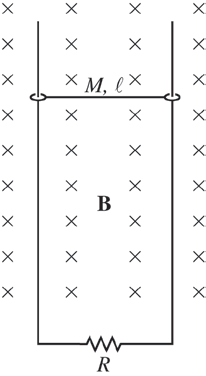
\includegraphics[scale=0.5]{images/img-014-034.png}
\end{figure}


\question
A bar of mass $M$ and length $\ell$ is connected to two long vertical frictionless rails. The bar and the rails have negligible resistance. They are placed in a uniform magnetic field of strength $B$ directed into the page as shown above. The bottoms of the rails are connected by a resistor of resistance $R$. The bar is released from rest in the position shown. Express all algebraic answers in terms of the given quantities and fundamental constants. % 请删除并替换本行,与上一行 \question 之间不要留空行

\begin{parts}

%-------------------------------------------------------------------------------
% 请勿删除本注释
% Part (a)
%
% 指引:
% 如在小问之前有通用问题描述,请放置于此
%-------------------------------------------------------------------------------

\part
Indicate on the diagram the direction of the current in the resistor. % 请删除并替换本行,与上一行 \part 之间不要留空行

At a particular time $T$, the bar is falling with speed $v_{1}$ but has not yet reached the bottom of the magnetic field.

%-------------------------------------------------------------------------------
% 请勿删除本注释
% Part (b)
%
% 指引:
% 如在小问之前有通用问题描述,请放置于此
%-------------------------------------------------------------------------------

\part
Calculate the power dissipated as heat in the resistor at time $T$. % 请删除并替换本行,与上一行 \part 之间不要留空行

%-------------------------------------------------------------------------------
% 请勿删除本注释
% Part (c)
%
% 指引:
% 如在小问之前有通用问题描述,请放置于此
%-------------------------------------------------------------------------------

\part
Calculate the magnitude of the magnetic force on the bar at time $T$ and state its direction. % 请删除并替换本行,与上一行 \part 之间不要留空行

At some time before leaving the magnetic field, the bar reaches a terminal velocity.

%-------------------------------------------------------------------------------
% 请勿删除本注释
% Part (d)
%
% 指引:
% 如在小问之前有通用问题描述,请放置于此
%-------------------------------------------------------------------------------

\part
Determine this terminal velocity. % 请删除并替换本行,与上一行 \part 之间不要留空行

%-------------------------------------------------------------------------------
% 请勿删除本注释
% Part (e)
%
% 指引:
% 如在小问之前有通用问题描述,请放置于此
%-------------------------------------------------------------------------------

\part
Write, but do NOT solve, the differential equation for the velocity of the falling bar while it is in the magnetic field. % 请删除并替换本行,与上一行 \part 之间不要留空行

%-------------------------------------------------------------------------------
% 请勿删除本注释
% Part (f)
%
% 指引:
% 如在小问之前有通用问题描述,请放置于此
%-------------------------------------------------------------------------------

\part
A second identical resistor is placed in parallel with the first. Is the terminal velocity reached by the bar in this case greater than, less than, or equal to that in part (d)? % 请删除并替换本行,与上一行 \part 之间不要留空行

\underline{\qquad} Greater than  \qquad  \underline{\qquad} Less than  \qquad     \underline{\qquad} Equal to

Justify your answer.


\end{parts}
